\subsection{Opgaver}

\begin{enumerate}
	\item Lad $f(x)=12x-3$, $ g(x)=-x^2-3x+1$ og bestem 
	\begin{align*}
	f\Big(-\frac{1}{3}\Big),&&f(-1),&& (f+g)(-2).
	\end{align*} 
	Bestem også $x$ så $f(x)=0$.
	
	\item \label{it:poly1} På Figur~\ref{fig:poly1} ses graferne for funktionerne
	\begin{align*}
		f(x)=x-2,&& g(x)=-\frac{1}{2}x+1,&&h(x)=5x+9.
	\end{align*}
	Bestem hvilke grafer hører til hvilke funktioner.
	\begin{figure}
		\centering
		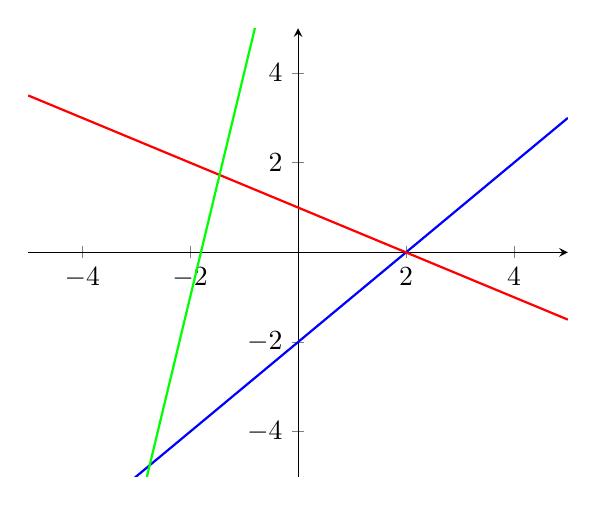
\begin{tikzpicture}
		\begin{axis}[xmin=-5,xmax=5,ymin=-5,ymax=5,axis x line=center,
		axis y line=center]
			\addplot[thick,blue] {x-2};
			\addplot[thick,red] {-x/2+1};
			\addplot[thick,green] {5*x+9};
		\end{axis}
		\end{tikzpicture}
		\caption{Opgave~\ref{it:poly1}}
		\label{fig:poly1}
	\end{figure}
	
	\item Bestem toppunktet for polynomiet $-2x^2+3x-1$
	
	\item Bestem hjørnepunkterne i den trekant som ses i Figur~\ref{fig:poly1}.
	
	\item Grafen for funktionen $f(x)=ax+b$ går gennem punkterne $(-1,3)$ og $(2,-1)$. Bestem $a$ og $b$.
	
	\item Lad $f(x)=2x-3$ og bestem $x_0$ så $ f(x_0)=x_0 $.
	
	\item Lad $ f(x)=\frac{3}{4}x^2-7x+5 $ og bestem først $f(-2)$ og derefter alle $x_0$ så $ f(x_0)=x_0 $
	
	\item Bestem koefficienterne $b$ og $c$ således at $f(x)=-x^2+bx+c$ har rødder $-2$ og $3$.
	
	\item Bestem et andengradspolynomium som går gennem punkterne $(-1,2)$, $(1,-1)$, $(2,4)$
	
	\item Bestem skæringspunkterne mellem $f(x)=2x^3-x^2+x-1$ og $h(x)=2x-1$.
	
	\item \label{it:poly2} På Figur~\ref{fig:poly2} ses grafen for et andengradspolynomium $f(x)=ax^2+bx+c$. Bestem fortegnene for $a,b,c,d$ ud fra grafen ($d$ betegner diskriminanten).
	
	\begin{figure}
		\centering
		\begin{tikzpicture}
		\begin{axis}[xmin=-1,xmax=2,ymin=-2,ymax=3,axis x line=center,
		axis y line=center,ticks=none]
			\addplot[thick,blue,samples=200]{2*x^2-2*x-1};
		\end{axis}
		\end{tikzpicture}
		\caption{Opgave~\ref{it:poly2}}
		\label{fig:poly2}
	\end{figure}
	
	\item \label{it:poly3} Figur~\ref{fig:poly3} viser skæringerne mellem $f(x)=2x^3-x^2-3x+2$ og $g(x)=-x^2-x+2$. Bestem skæringspunkterne mellem disse to polynomier.
	\begin{figure}
		\centering
		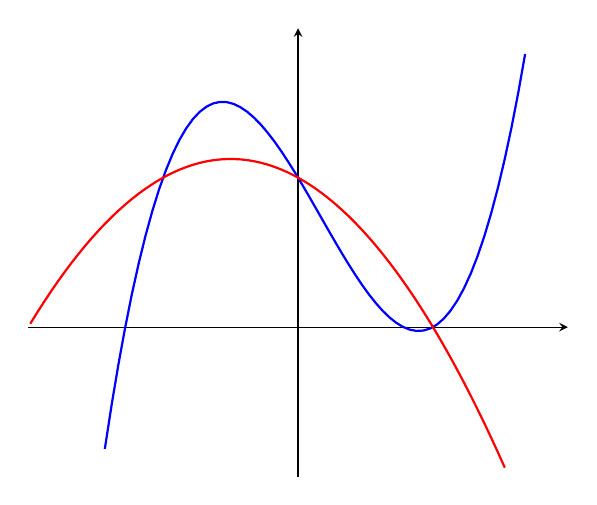
\begin{tikzpicture}
		\begin{axis}[xmin=-2,xmax=2,ymin=-2,ymax=4,axis x line=center,
		axis y line=center,ticks=none,restrict y to domain=-2:4,restrict x to domain=-2:2]
		\addplot[blue,thick,samples=200] {2*x^3-x^2-3*x+2};
		\addplot[red,thick,samples=200] {-x^2-x+2};]
		\end{axis}
		\end{tikzpicture}
		\caption{Opgave~\ref{it:poly3}}
		\label{fig:poly3}
	\end{figure}
	

	
	\item Lad $f(x)=2x^2-bx+1$ (se \href{https://www.geogebra.org/m/B5GvWyYW}{GeoGebra}) og bestem
	\begin{enumerate}
		\item For hvilke værdier af $b$ ligger toppunktet for $f$ i første kvadrant?
		\item For hvilke værdier af $b$ ligger toppunktet for $f$ i tredje kvadrant?
	\end{enumerate}
	
	\item Lad $a_0$ og $c_0$ være faste tal og lad $f(x)=a_0 x^2+bx+c_0$ være et polynomium hvor $b$ er vilkårlig. Vis, at toppunktet for $f$ ligger på parablen $-a_0 x^2+c_0$ uanset værdien af $b$. Se eventuelt \href{https://www.geogebra.org/m/B5GvWyYW}{GeoGebra}
\end{enumerate}